% RESULTS - AUTO-UPDATED SECTION
% This section is scaffolded for the RQ-driven paper suite.
% It will be populated with findings once experiments run.

\newcommand{\pl}[1]{\textcolor{gray}{#1}}

\subsection{Overview}

We present results from the curated paper suite (baseline, calibration, ablations, sensitivity,
and RQ-specific experiments). Table~\ref{tab:summary} provides a high-level overview.

\begin{table}[htbp]
\centering
\caption{Summary of experimental results (placeholder)}
\label{tab:summary}
\begin{tabular}{lrrr}
\toprule
Experiment & Configurations & Total Runs & Key Finding \\
\midrule
\pl{Baseline} & \pl{--} & \pl{--} & \pl{TBD} \\
\pl{Calibration} & \pl{--} & \pl{--} & \pl{TBD} \\
\pl{Ablation} & \pl{--} & \pl{--} & \pl{TBD} \\
\pl{Sensitivity} & \pl{--} & \pl{--} & \pl{TBD} \\
\bottomrule
\end{tabular}
\end{table}

% ============================================================================
\subsection{RQ3: Proposal Pipeline Effects}
% ============================================================================

\subsubsection{Findings}

\begin{figure}[htbp]
    \centering
    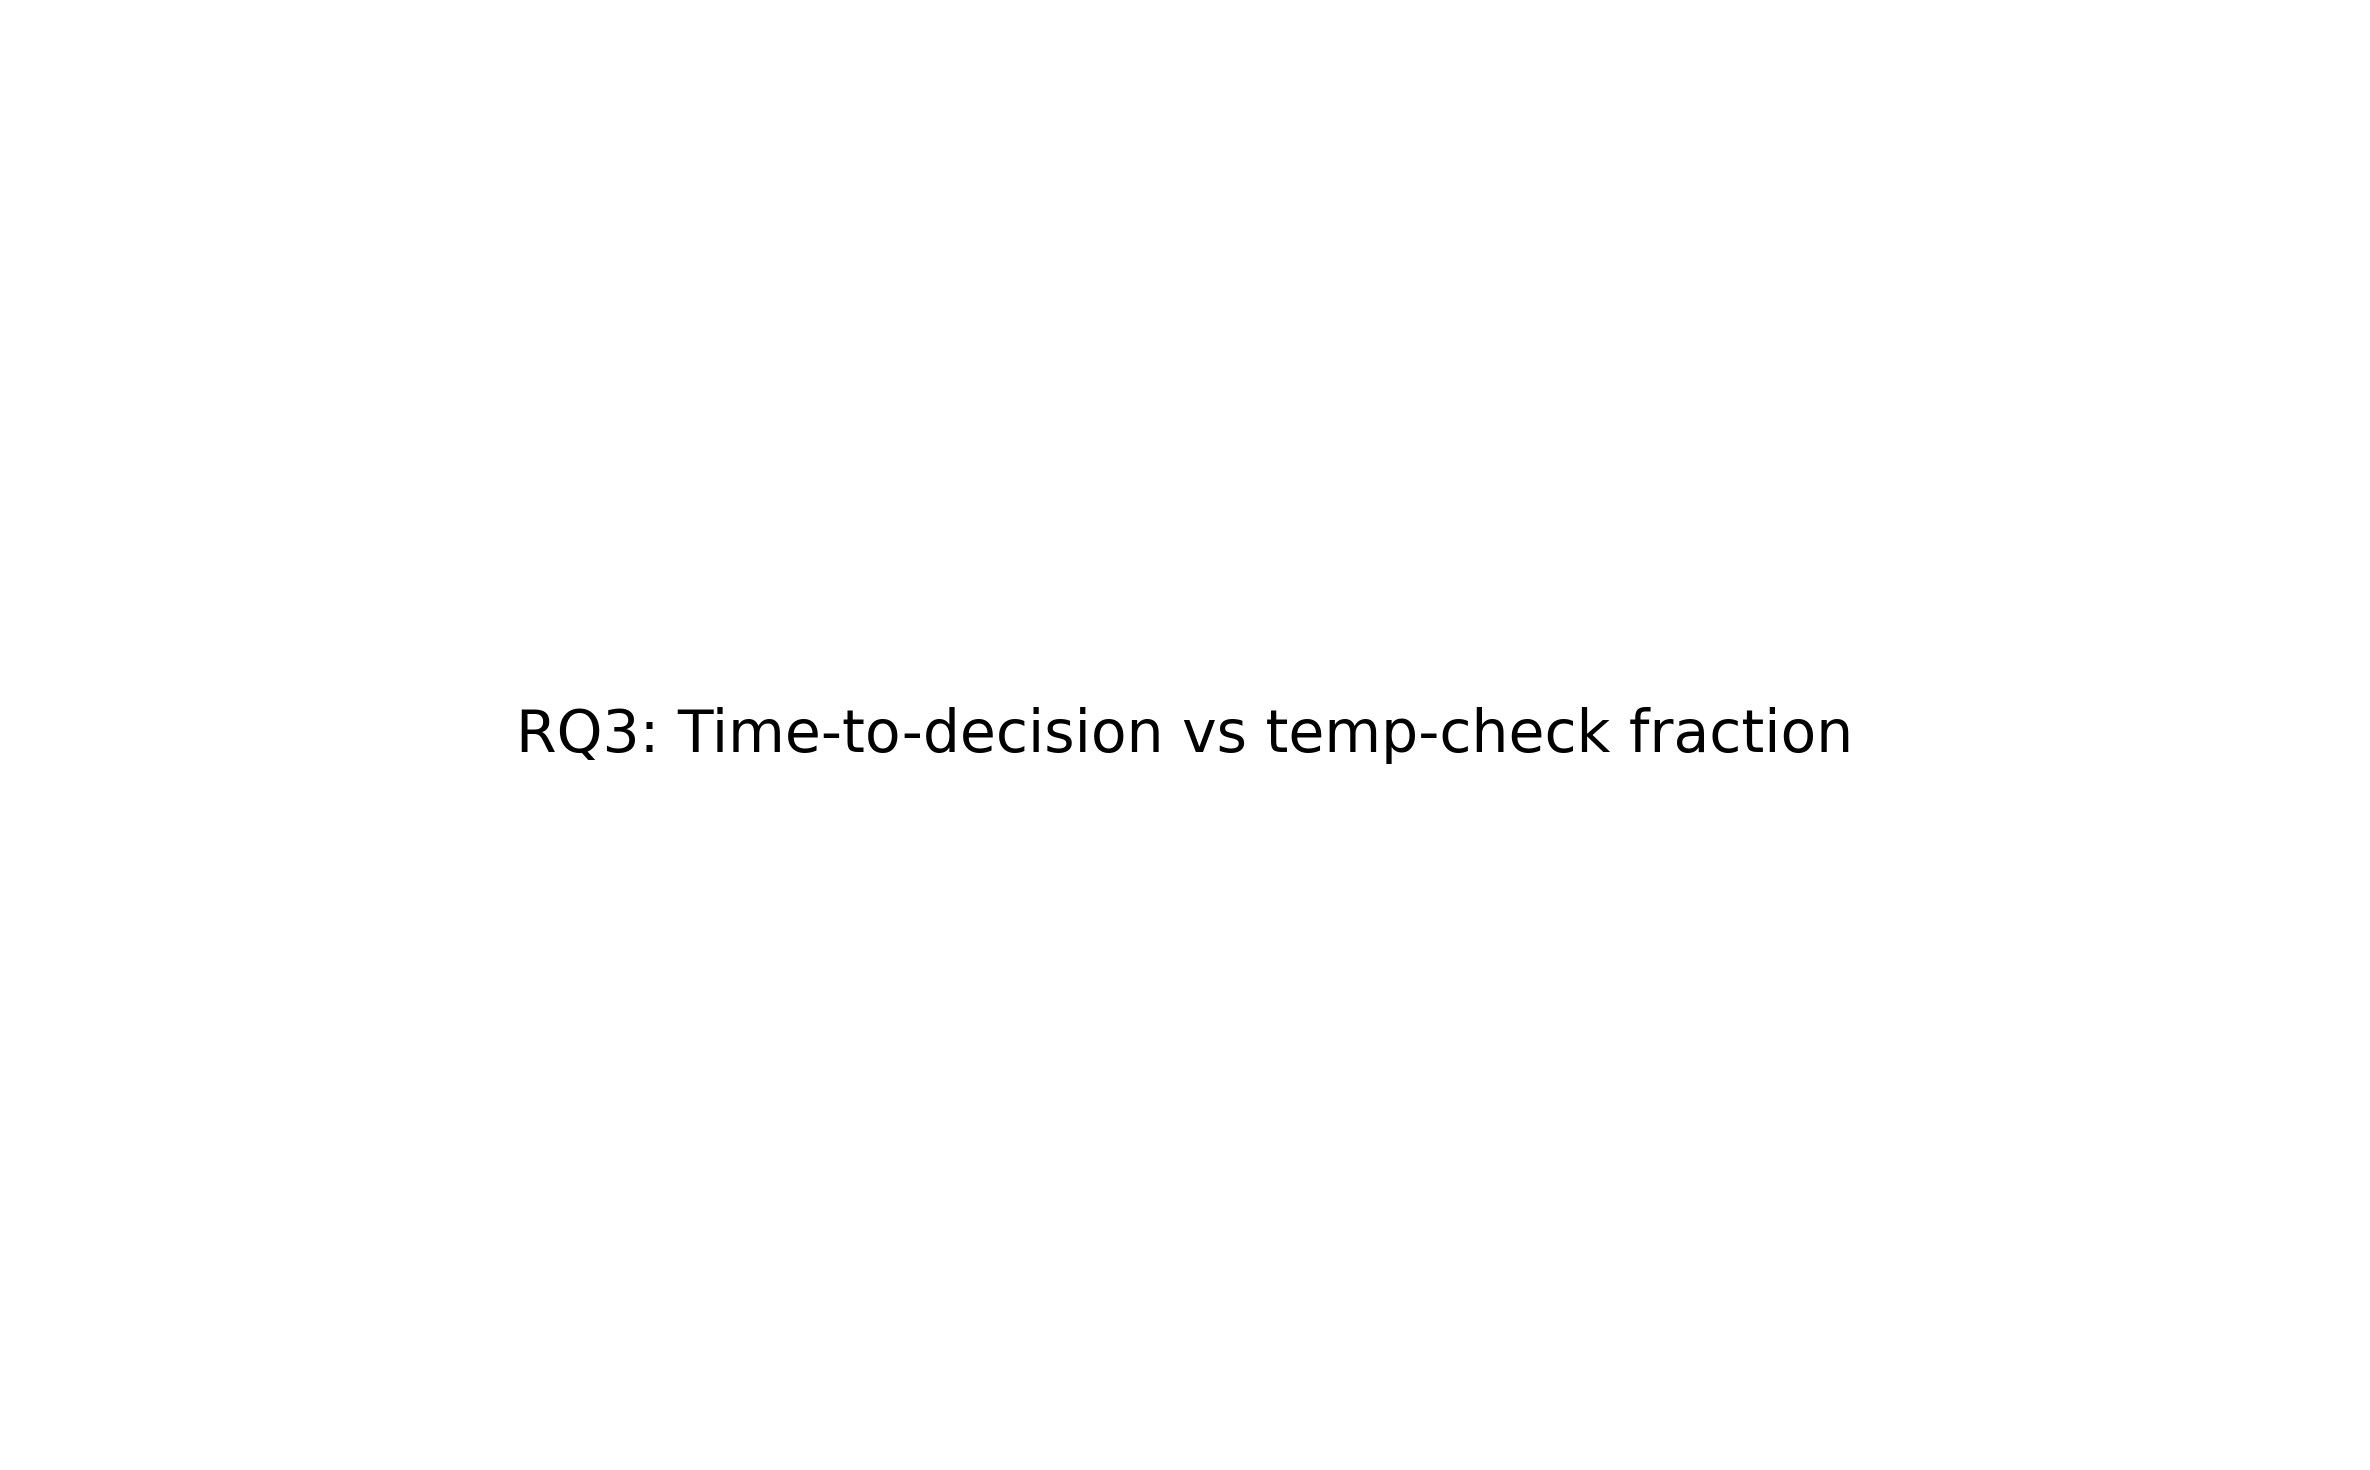
\includegraphics[width=0.8\textwidth]{figures/rq3_time}
    \caption{Decision time vs temp-check fraction (placeholder).}
    \label{fig:rq3-time}
\end{figure}

\begin{figure}[htbp]
    \centering
    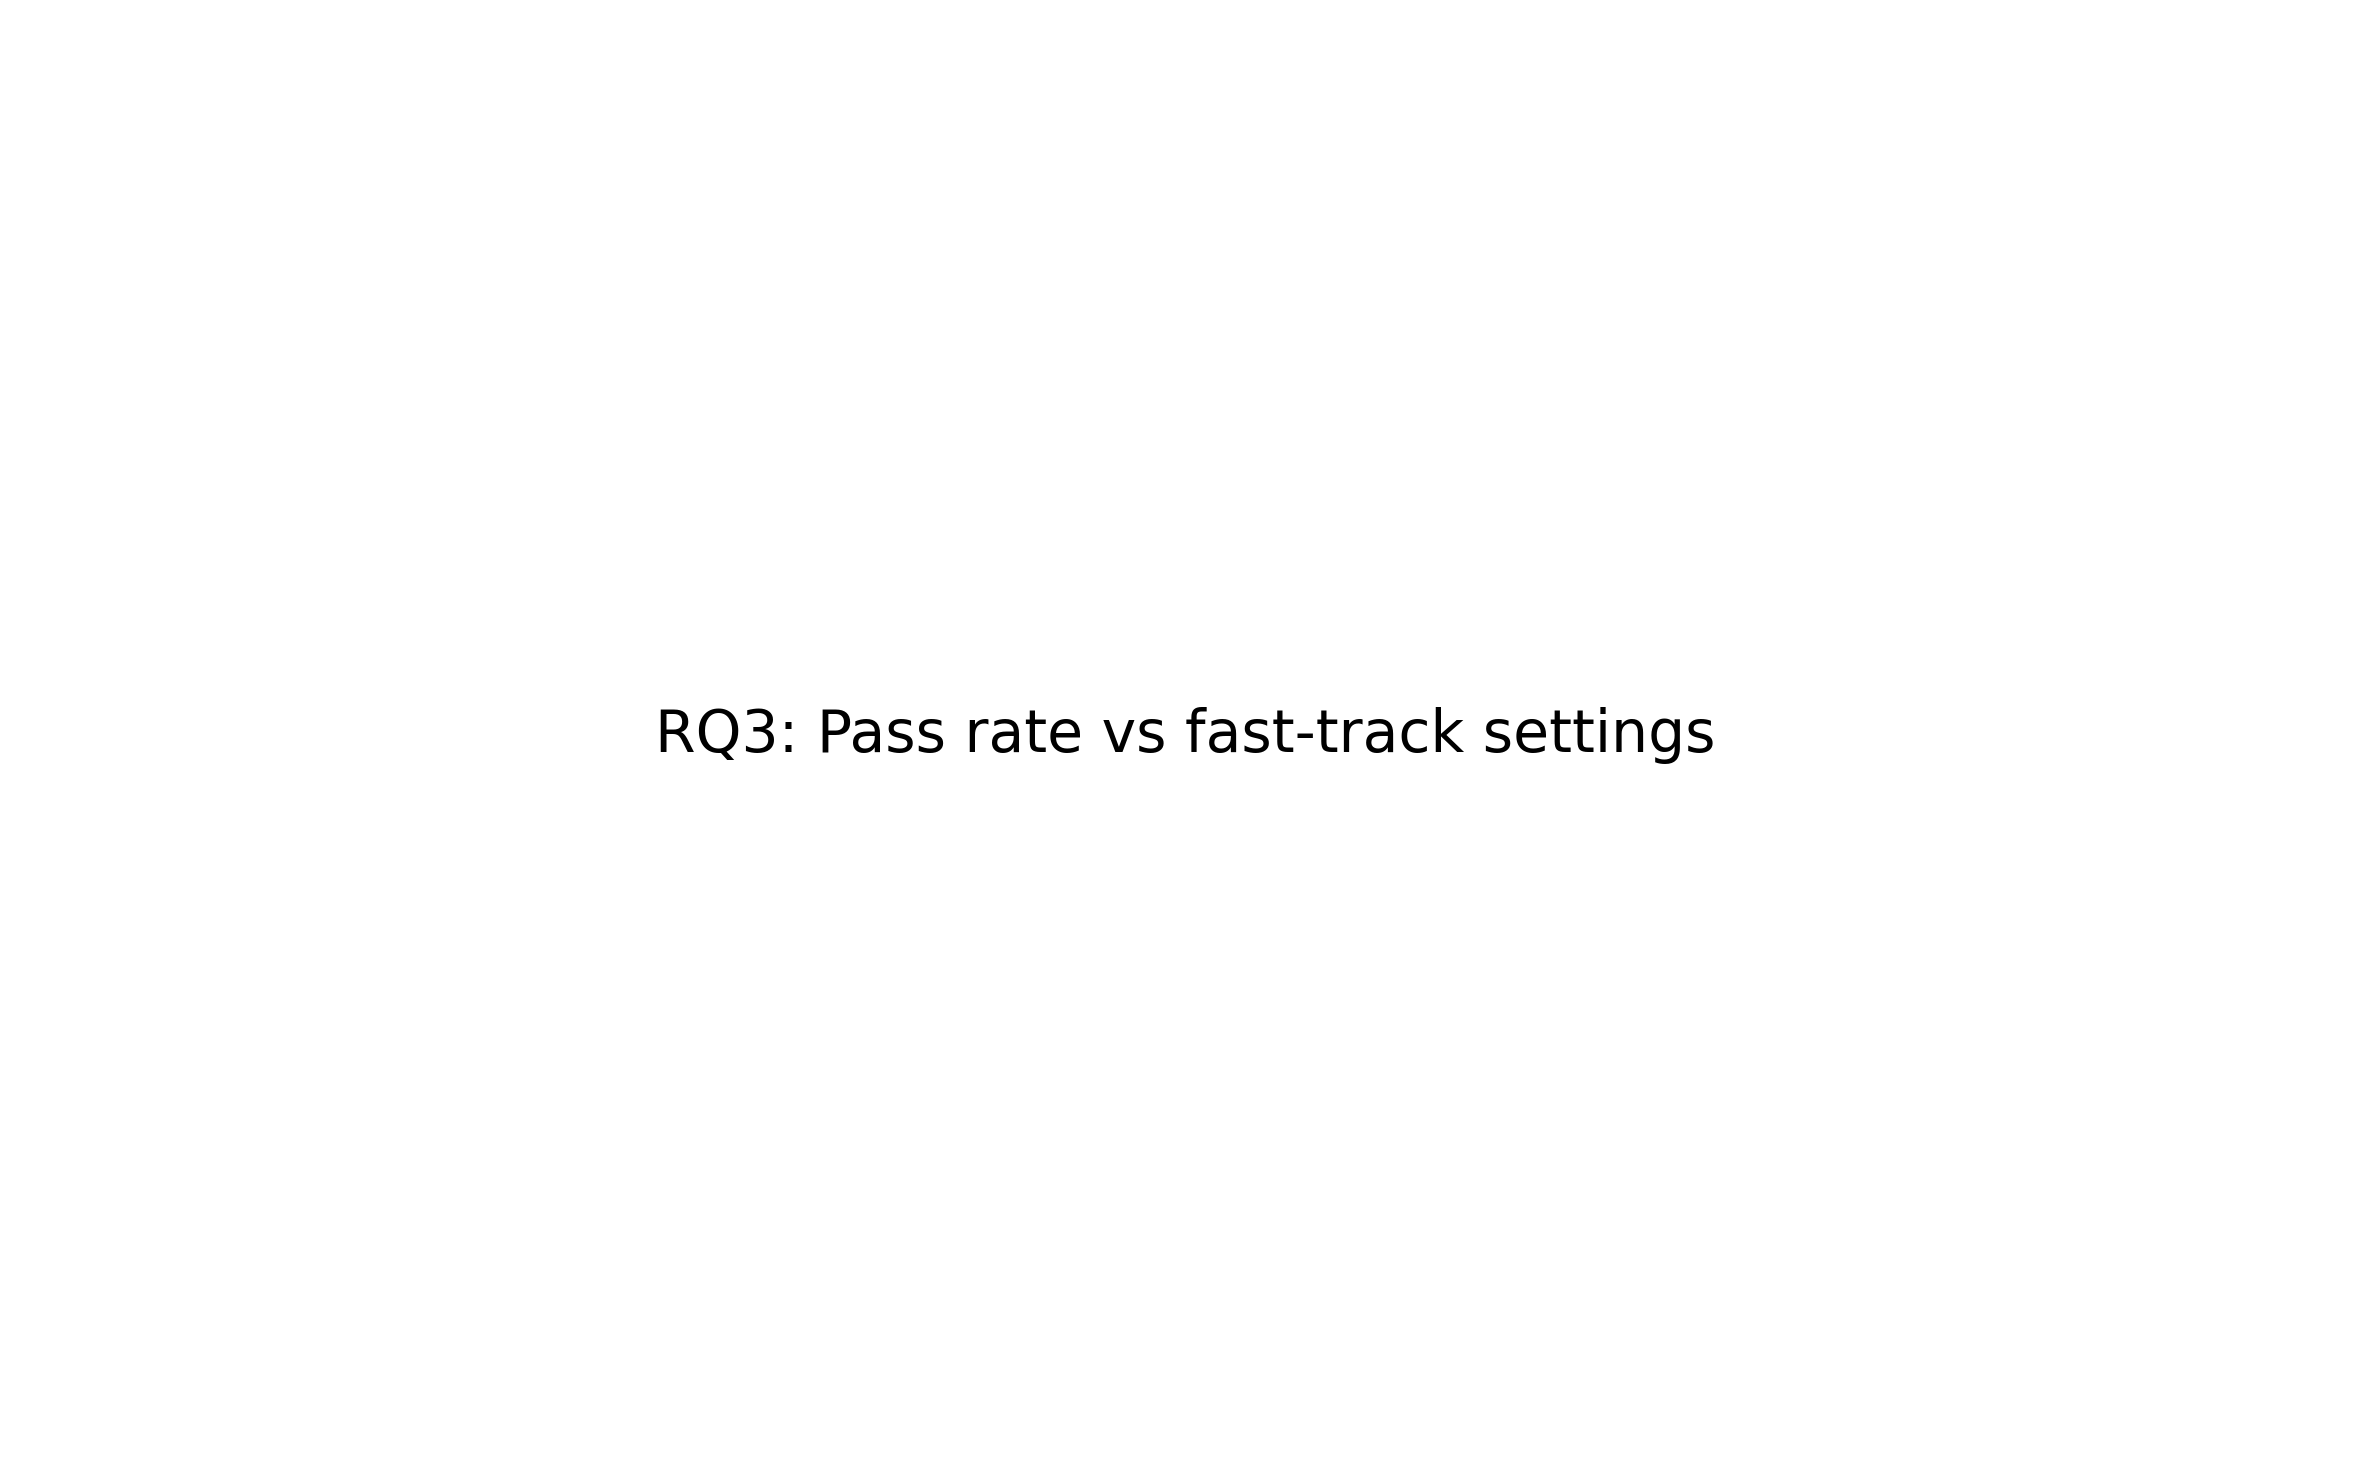
\includegraphics[width=0.8\textwidth]{figures/rq3_passrate}
    \caption{Pass rate vs fast-track settings (placeholder).}
    \label{fig:rq3-passrate}
\end{figure}

\begin{table}[htbp]
\centering
\caption{Abandonment and quorum reach by pipeline settings (placeholder)}
\label{tab:rq3-summary}
\begin{tabular}{lccc}
\toprule
Config & Abandonment Rate & Quorum Reach & Pass Rate \\
\midrule
\pl{A} & \pl{--} & \pl{--} & \pl{--} \\
\pl{B} & \pl{--} & \pl{--} & \pl{--} \\
\pl{C} & \pl{--} & \pl{--} & \pl{--} \\
\bottomrule
\end{tabular}
\end{table}

% ============================================================================
\subsection{RQ4: Treasury Resilience}
% ============================================================================

\subsubsection{Findings}

\begin{figure}[htbp]
    \centering
    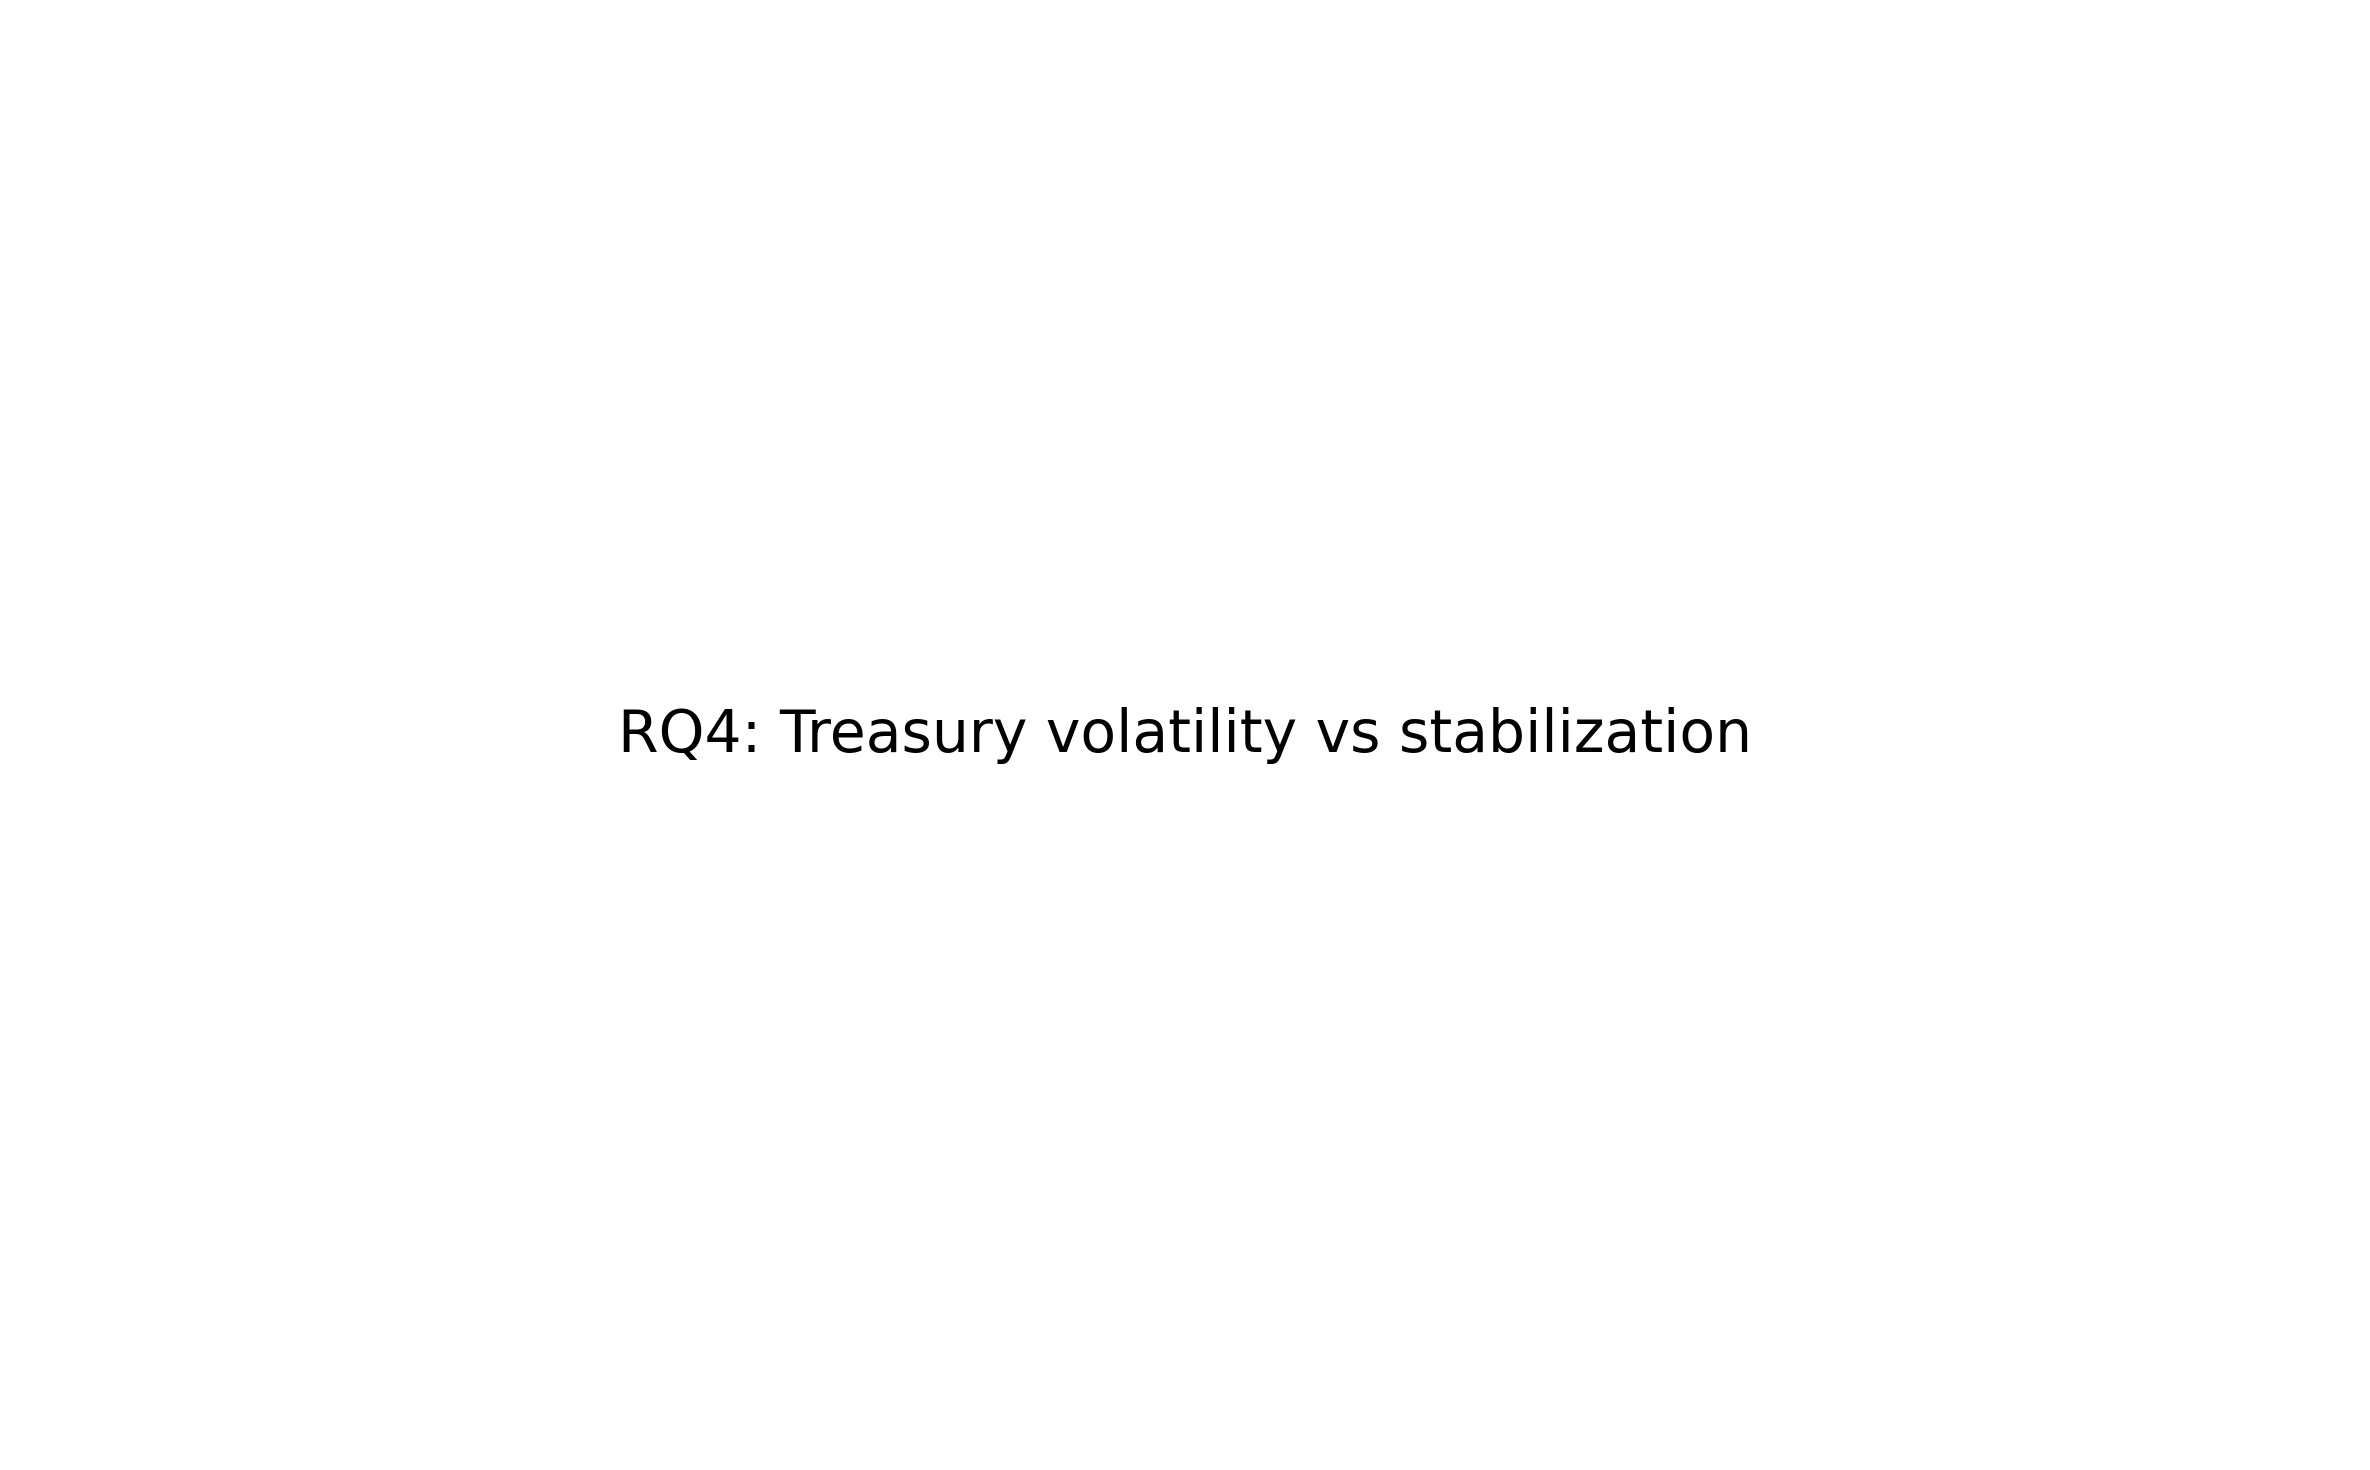
\includegraphics[width=0.8\textwidth]{figures/rq4_volatility}
    \caption{Treasury volatility under stabilization policies (placeholder).}
    \label{fig:rq4-volatility}
\end{figure}

\begin{figure}[htbp]
    \centering
    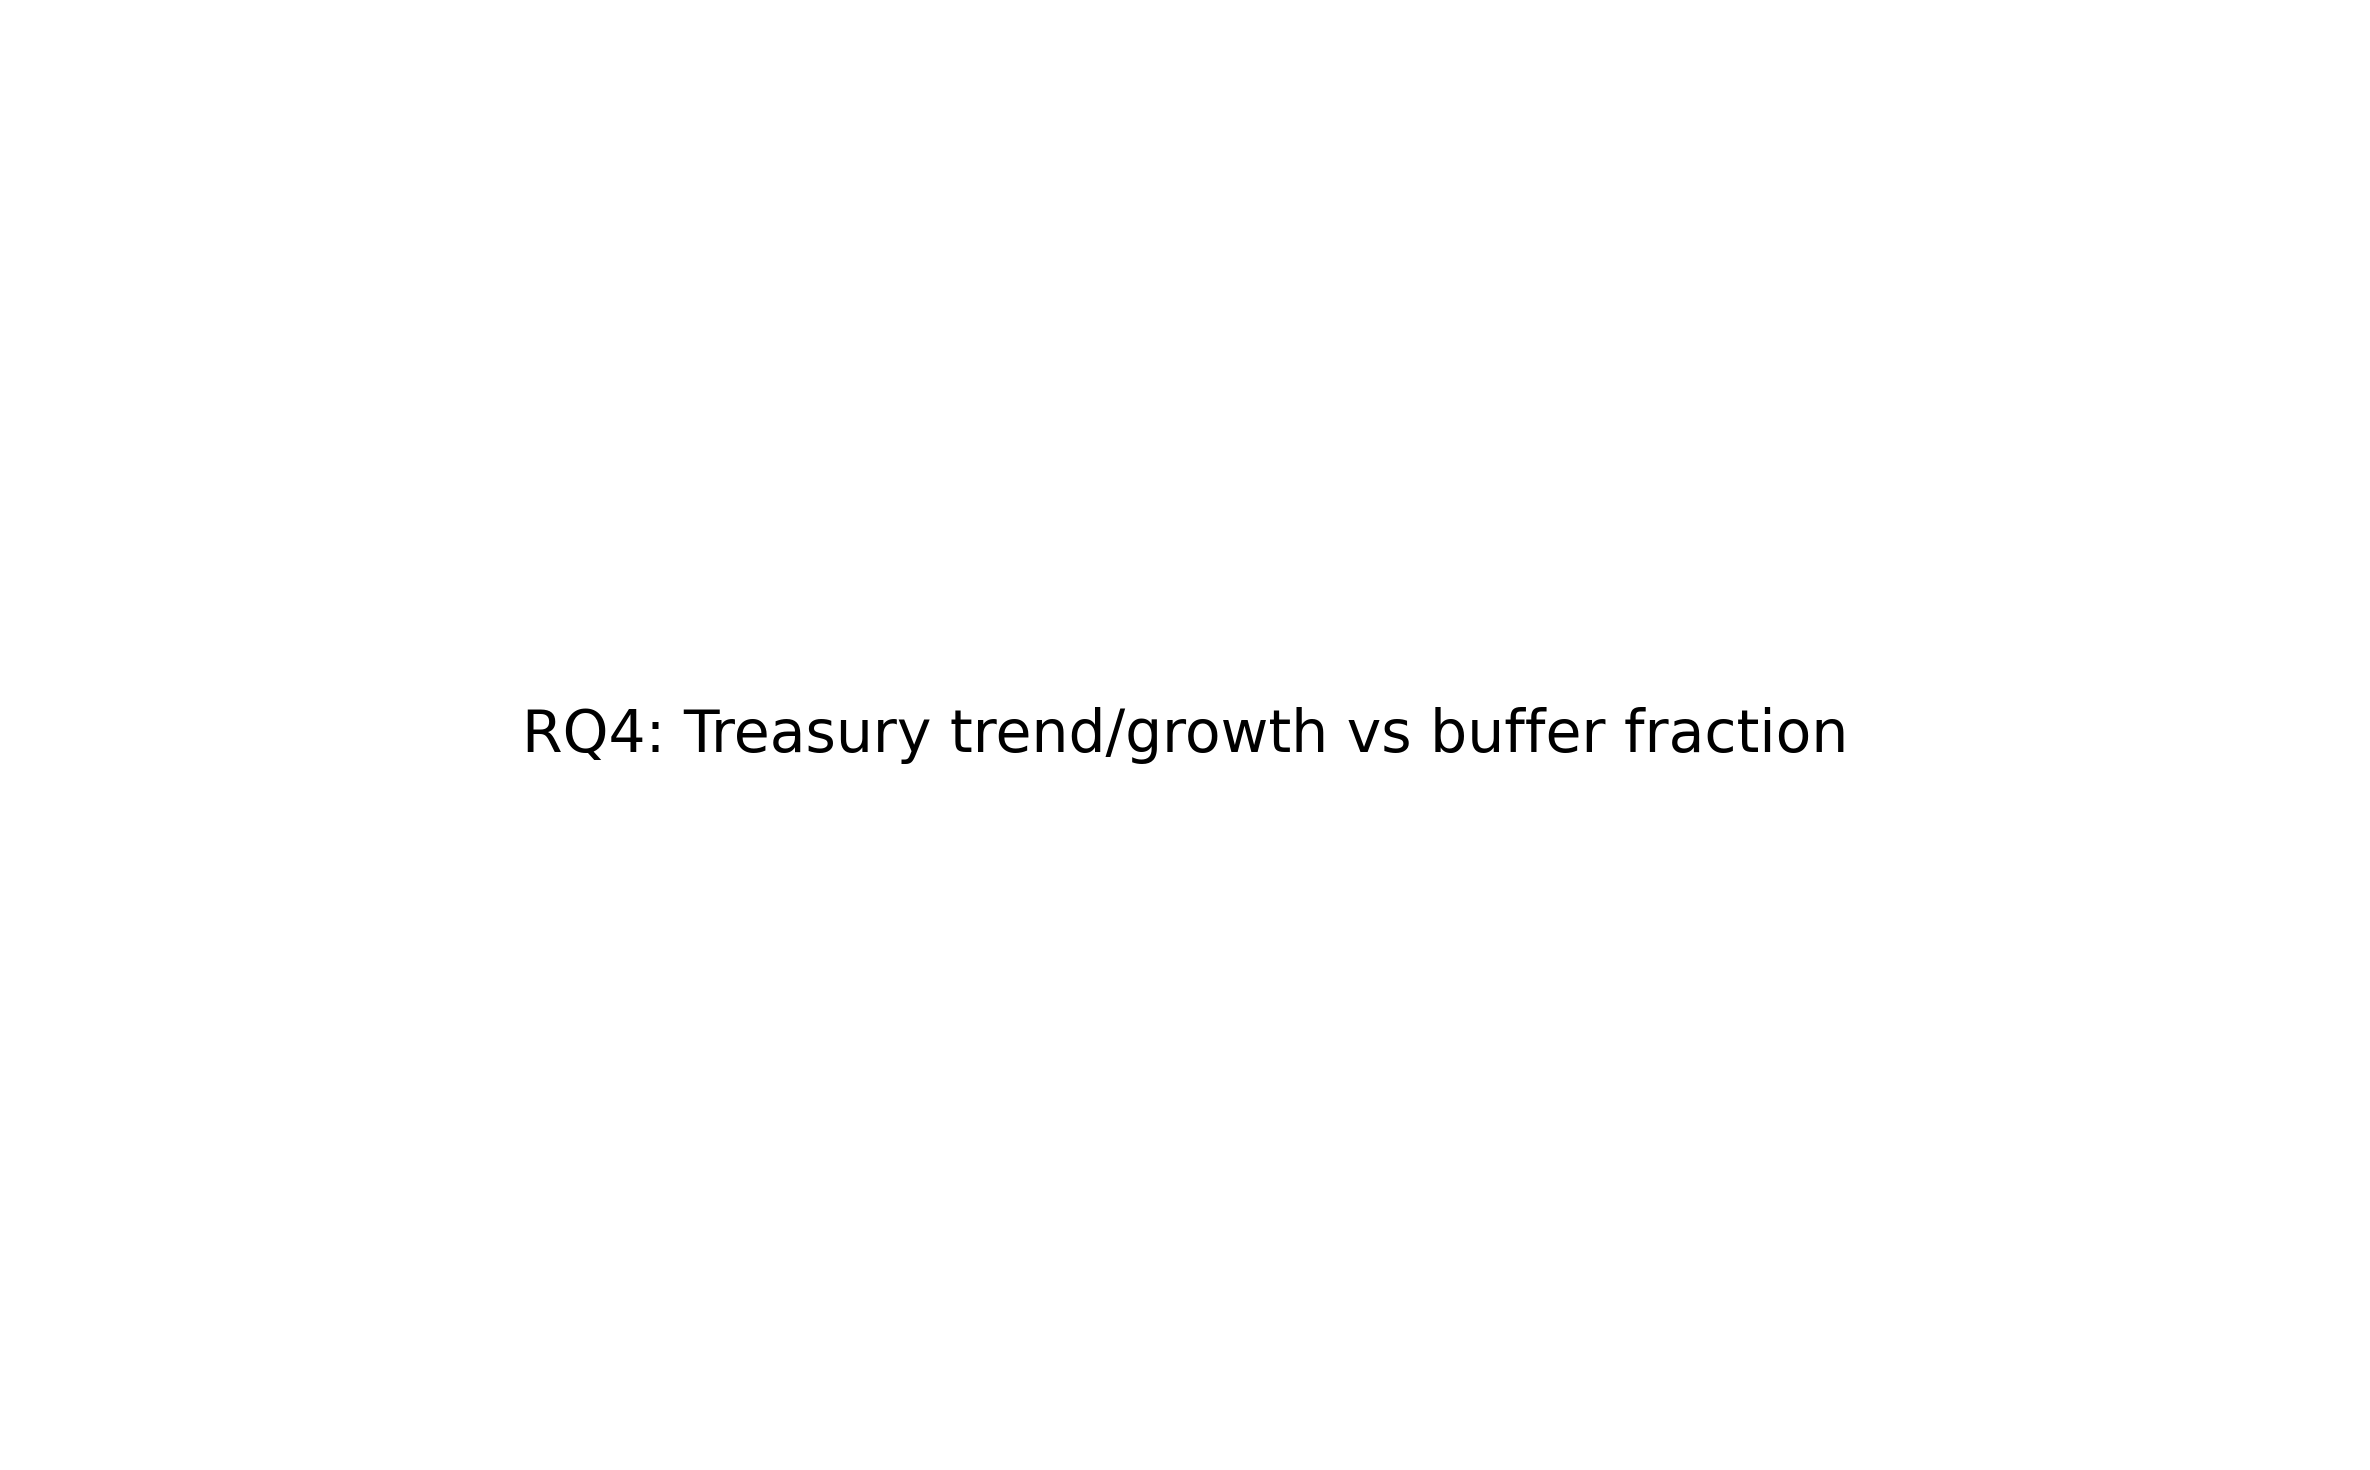
\includegraphics[width=0.8\textwidth]{figures/rq4_growth}
    \caption{Treasury trend/growth vs buffer fraction (placeholder).}
    \label{fig:rq4-growth}
\end{figure}

\begin{table}[htbp]
\centering
\caption{Final treasury and volatility by config (placeholder)}
\label{tab:rq4-summary}
\begin{tabular}{lccc}
\toprule
Config & Final Treasury & Volatility & Trend \\
\midrule
\pl{A} & \pl{--} & \pl{--} & \pl{--} \\
\pl{B} & \pl{--} & \pl{--} & \pl{--} \\
\pl{C} & \pl{--} & \pl{--} & \pl{--} \\
\bottomrule
\end{tabular}
\end{table}

% ============================================================================
\subsection{RQ5: Inter-DAO Cooperation}
% ============================================================================

\subsubsection{Findings}

\begin{figure}[htbp]
    \centering
    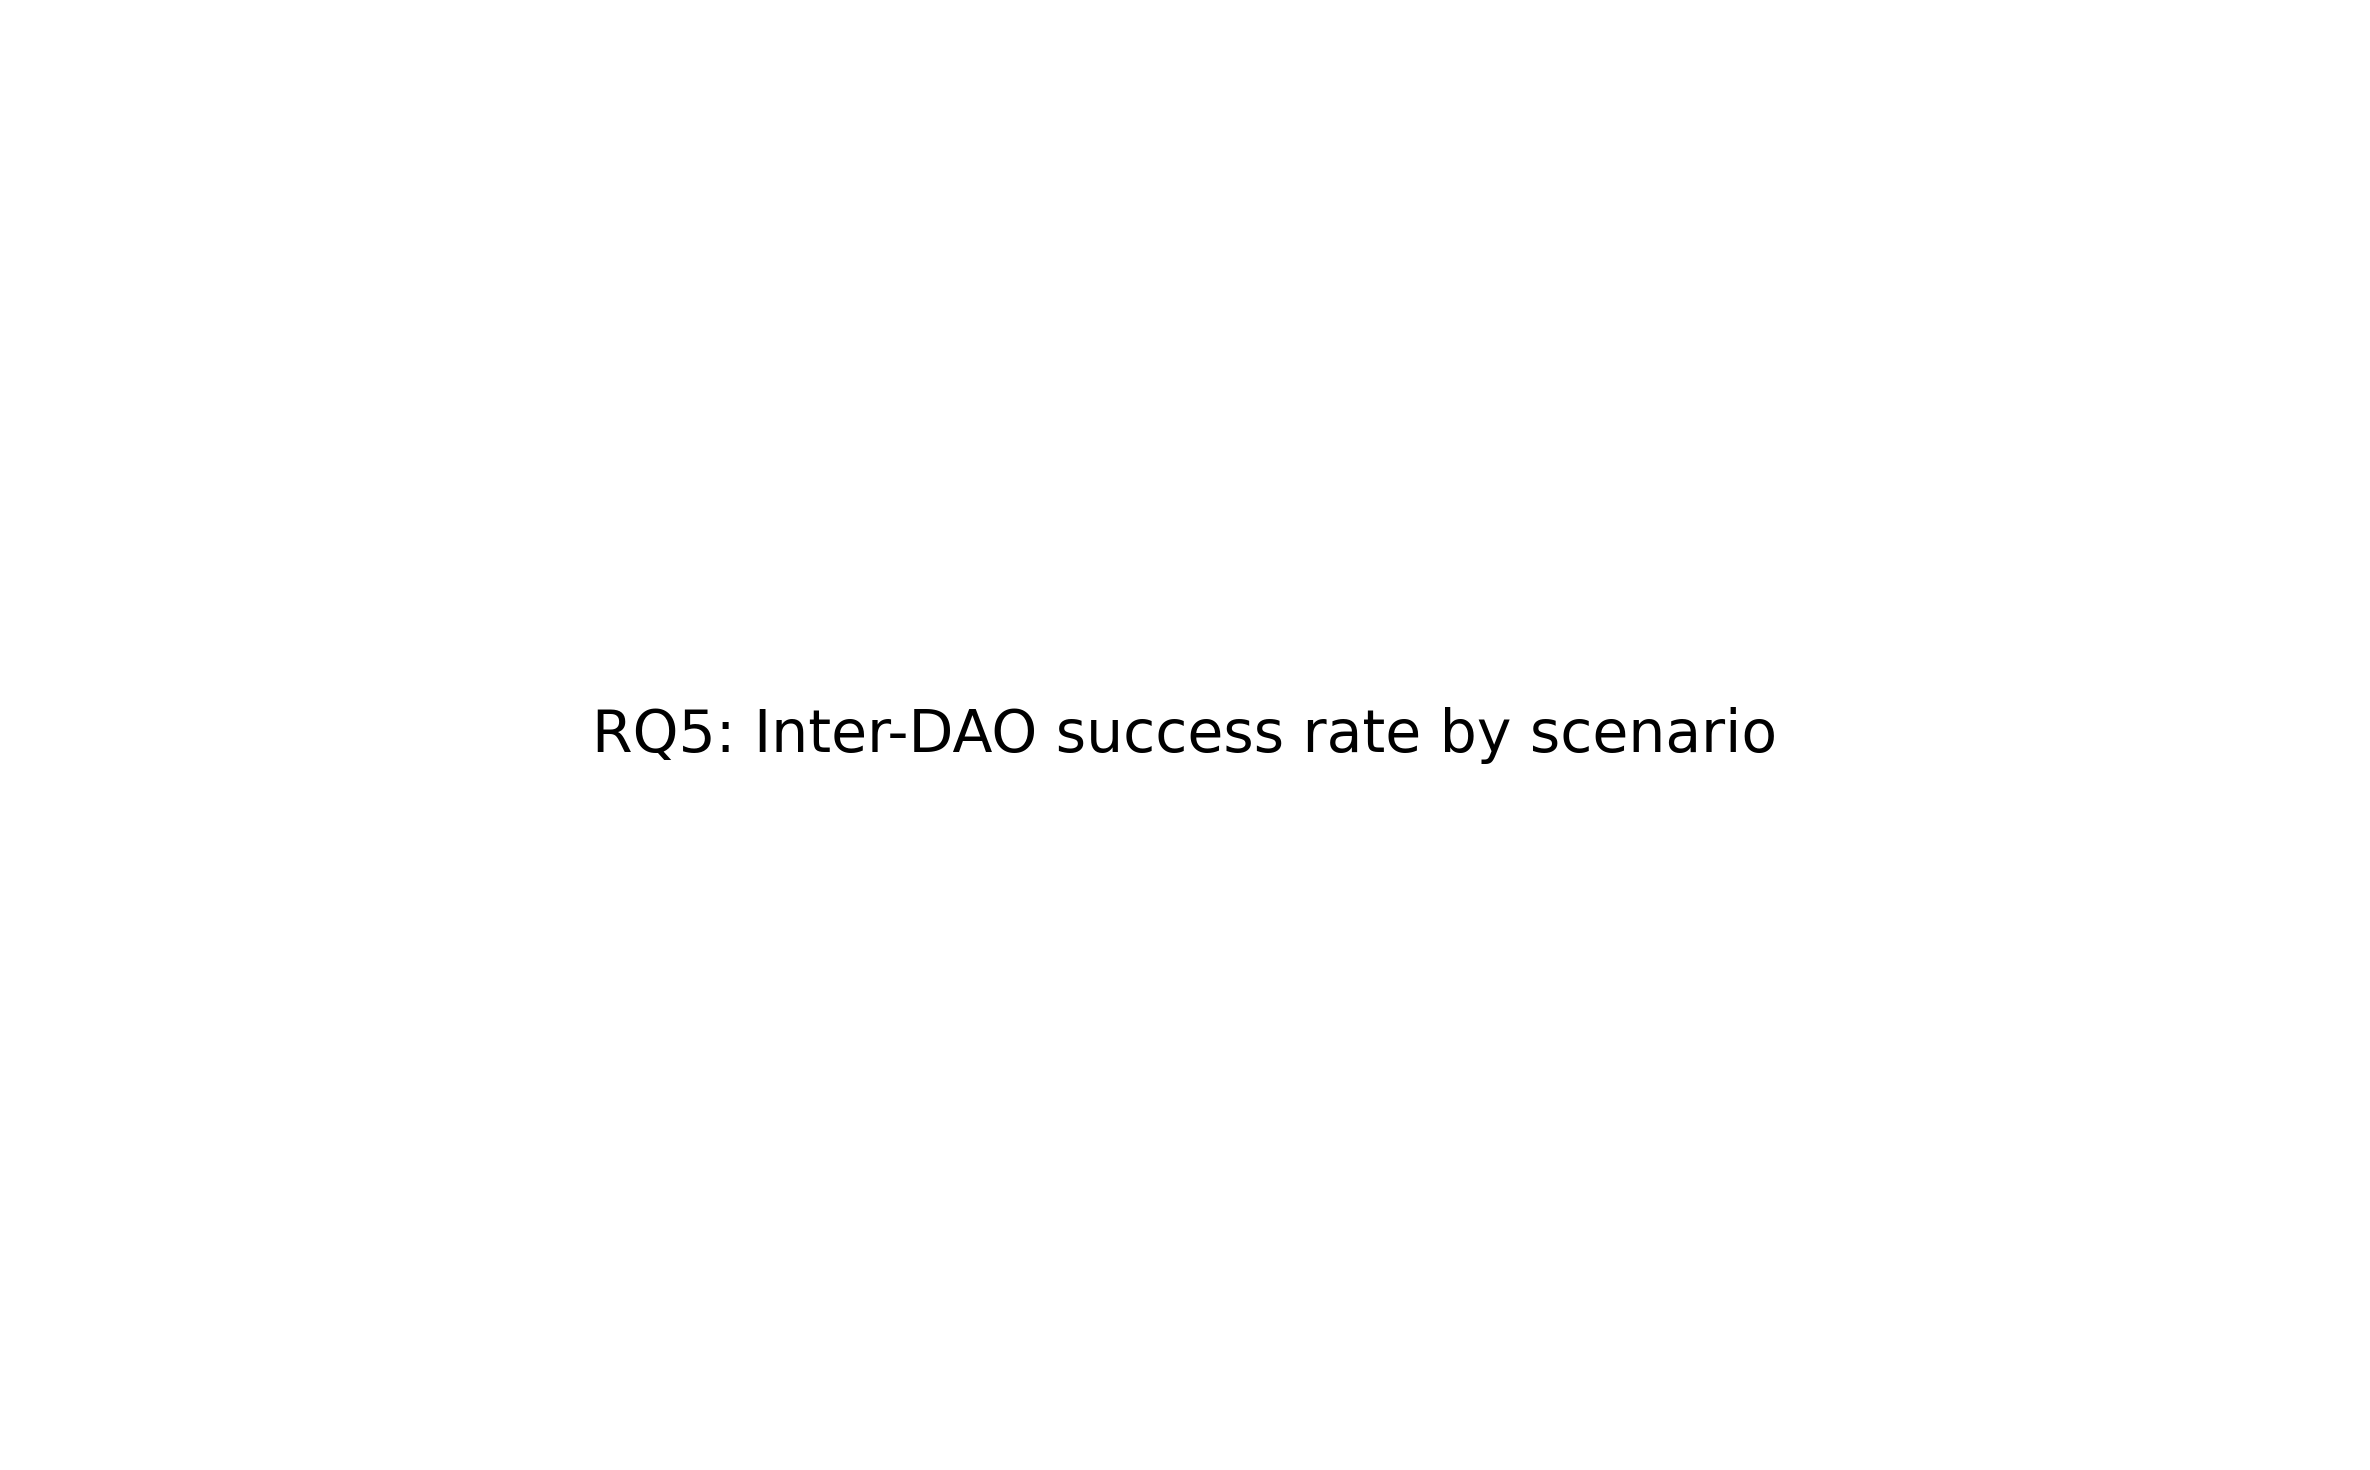
\includegraphics[width=0.8\textwidth]{figures/rq5_success}
    \caption{Inter-DAO success rate across scenarios (placeholder).}
    \label{fig:rq5-success}
\end{figure}

\begin{figure}[htbp]
    \centering
    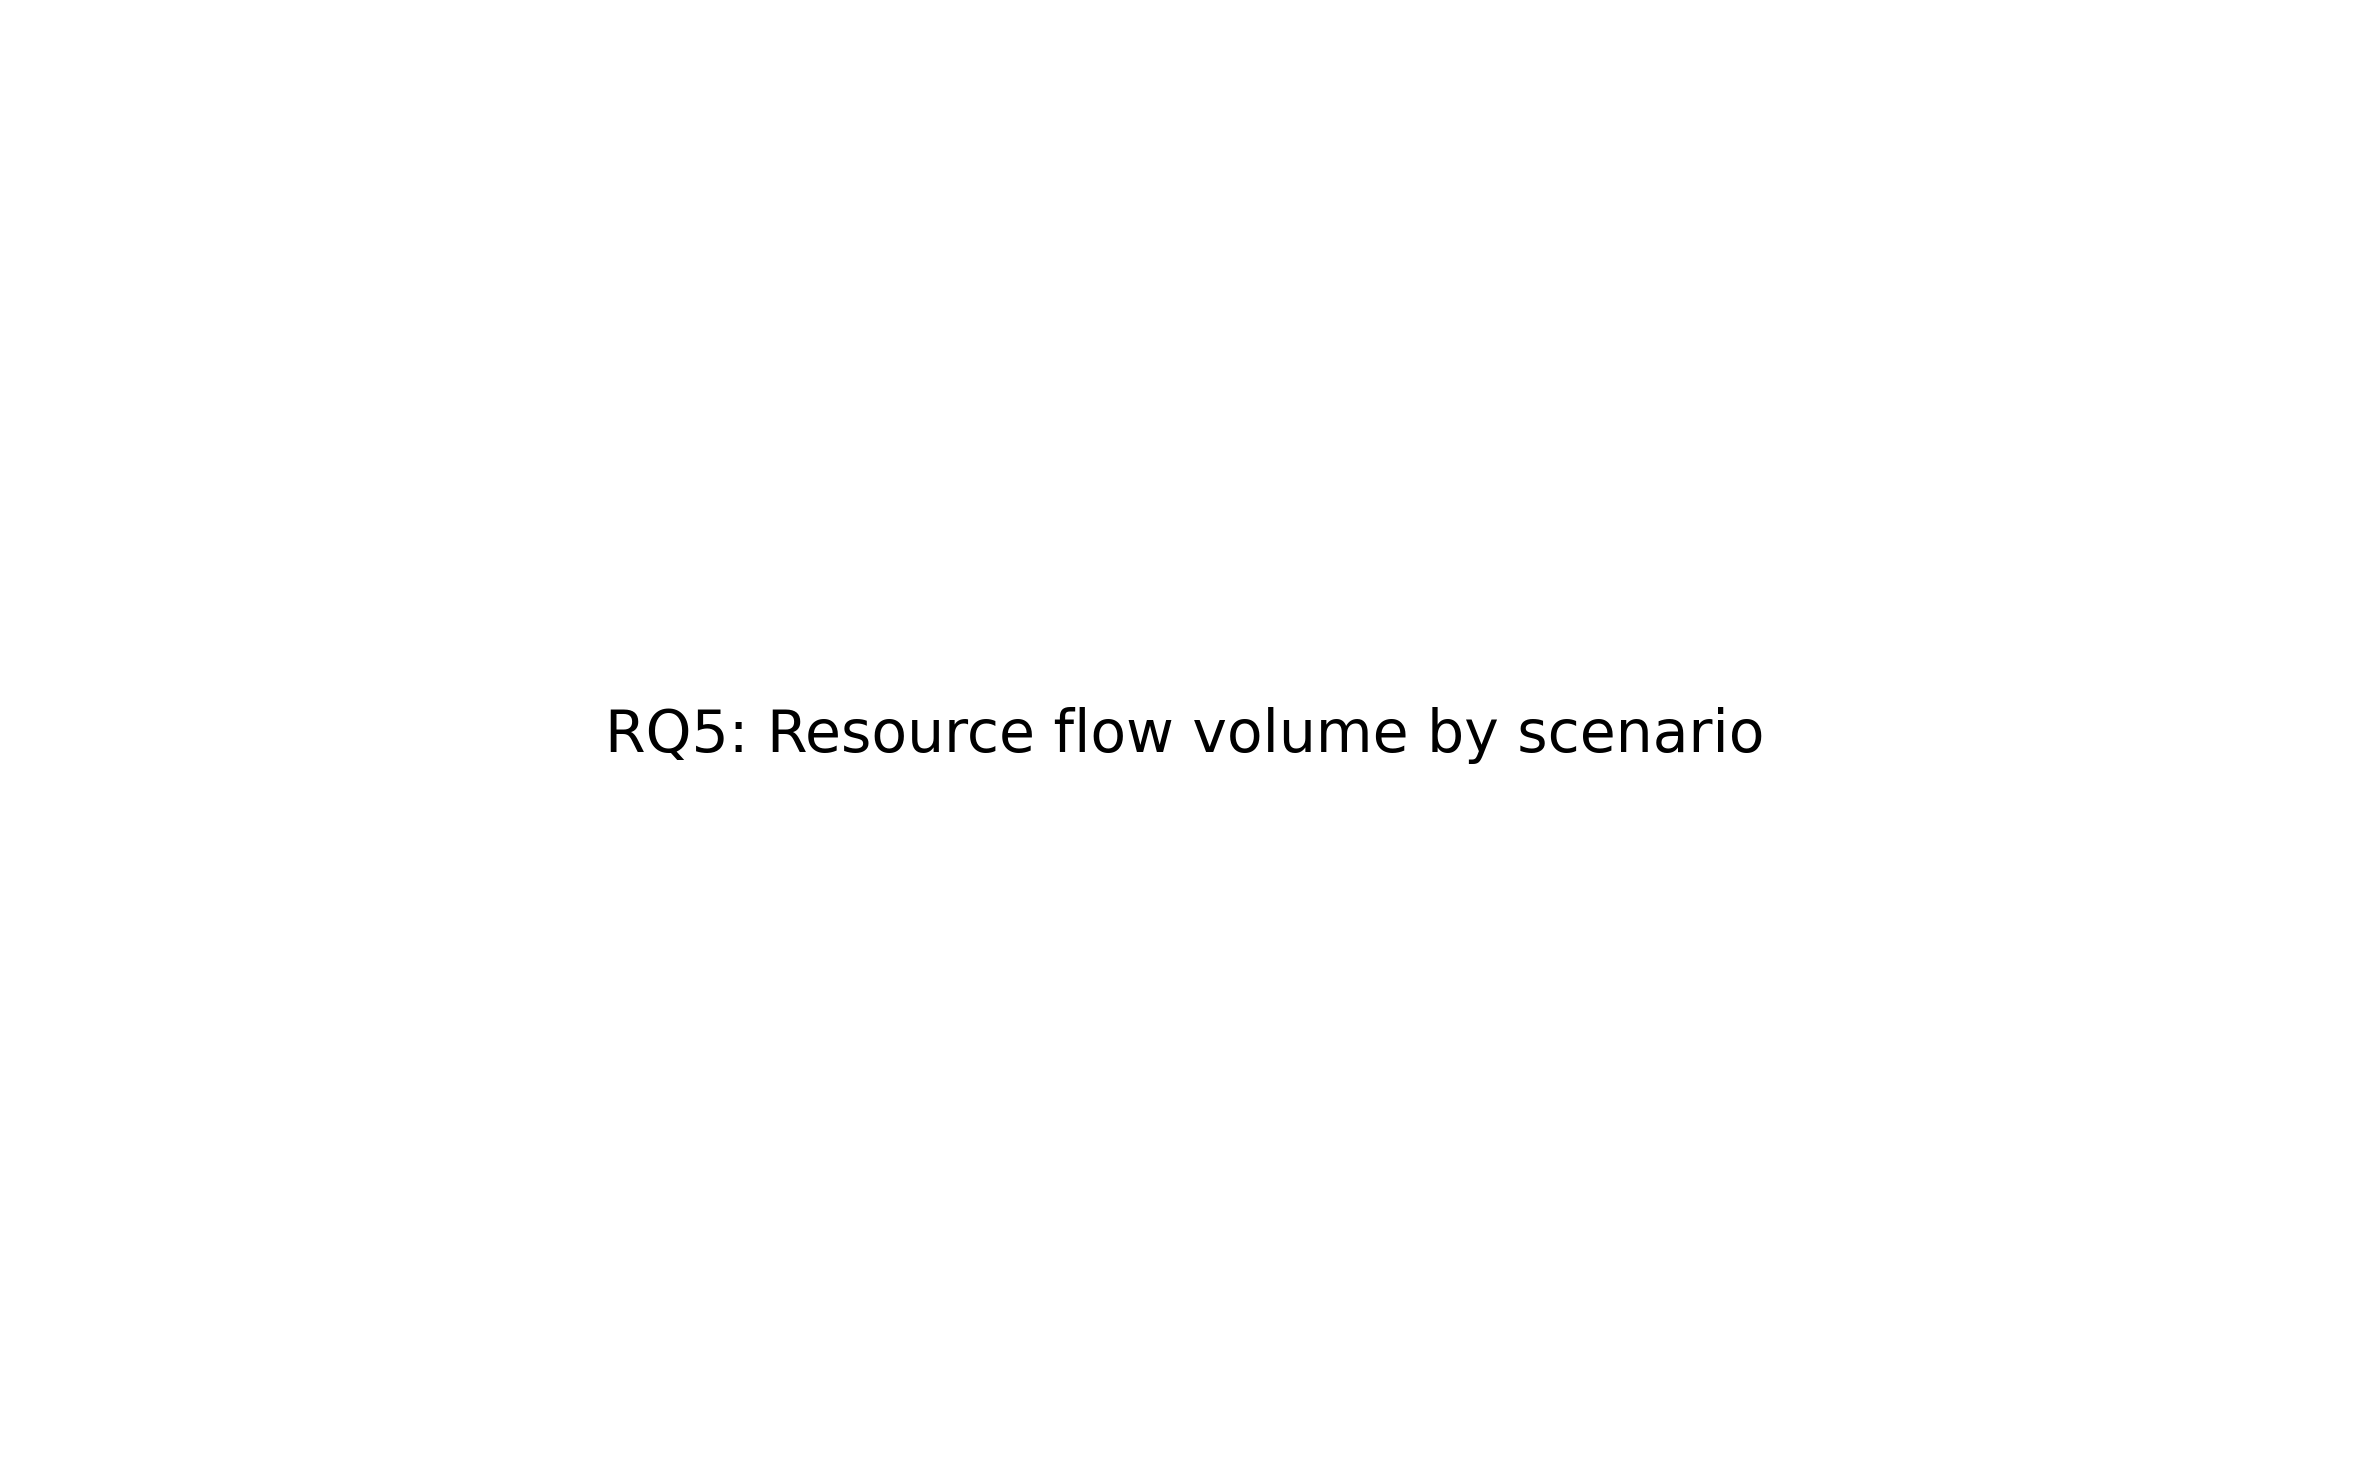
\includegraphics[width=0.8\textwidth]{figures/rq5_resources}
    \caption{Resource flow volume by scenario (placeholder).}
    \label{fig:rq5-resources}
\end{figure}

\begin{table}[htbp]
\centering
\caption{Cross-DAO alignment and shared budget summary (placeholder)}
\label{tab:rq5-summary}
\begin{tabular}{lccc}
\toprule
Scenario & Alignment & Shared Budget & Success Rate \\
\midrule
\pl{Homogeneous} & \pl{--} & \pl{--} & \pl{--} \\
\pl{Heterogeneous} & \pl{--} & \pl{--} & \pl{--} \\
\pl{Asymmetric} & \pl{--} & \pl{--} & \pl{--} \\
\bottomrule
\end{tabular}
\end{table}

% ============================================================================
\subsection{Baseline and Robustness}
% ============================================================================

\begin{table}[htbp]
\centering
\caption{Baseline headline metrics (placeholder)}
\label{tab:baseline-summary}
\begin{tabular}{lccc}
\toprule
Metric & Mean & Std & Notes \\
\midrule
\pl{Pass Rate} & \pl{--} & \pl{--} & \pl{--} \\
\pl{Turnout} & \pl{--} & \pl{--} & \pl{--} \\
\pl{Treasury Volatility} & \pl{--} & \pl{--} & \pl{--} \\
\bottomrule
\end{tabular}
\end{table}

% === AUTO-GENERATION METADATA ===
% Regenerate this section:
%   npm run paper:update -- --section results
% Source experiments: paper suite (placeholders until runs complete)
